\documentclass[10pt, a4paper]{article}

\usepackage[paper=a4paper, left=1.5cm, right=1.5cm, bottom=1.5cm, top=3.5cm]{geometry}
\usepackage[utf8]{inputenc}
\usepackage[T1]{fontenc}
\usepackage[spanish,es-noshorthands,es-ucroman]{babel}
\usepackage{indentfirst}
\usepackage{fancyhdr}
\usepackage{latexsym}
\usepackage{lastpage}
\usepackage[colorlinks=true, linkcolor=black]{hyperref}
\usepackage{calc}
\usepackage{a4wide}
\usepackage{listings}
\lstset{language={C++}, basicstyle=\small}
\usepackage{algorithm}
\usepackage{algorithmic}[1]
\usepackage{graphicx}
\usepackage{tikz}
\usepackage{amsmath}
\usepackage{framed}
\usepackage{amsfonts}
\usepackage{tkz-berge}
\usepackage{amsfonts}
\usepackage{color}
\usepackage{caratula}
\usepackage{cite}
\usepackage{paralist}


\definecolor{gray97}{gray}{.97}
\definecolor{gray75}{gray}{.75}
\definecolor{gray45}{gray}{.45}
%
% \lstset{ frame=Ltb,
% framerule=0pt,
% aboveskip=0.5cm,
% framextopmargin=3pt,
% framexbottommargin=3pt,
% framexleftmargin=0.4cm,
% framesep=0pt,
% rulesep=.4pt,
% backgroundcolor=\color{gray97},
% rulesepcolor=\color{black},
% %
% stringstyle=\ttfamily,
% showstringspaces = false,
% basicstyle=\small\ttfamily,
% commentstyle=\color{gray45},
% keywordstyle=\bfseries,
% %
% numbers=left,
% numbersep=15pt,
% numberstyle=\tiny,
% numberfirstline = false,
% breaklines=true,
% }
% % minimizar fragmentado de listados
% \lstnewenvironment{listing}[1][]
% {\lstset{#1}\pagebreak[0]}{\pagebreak[0]}
% \lstdefinestyle{consola}
% {basicstyle=\scriptsize\bf\ttfamily,
% backgroundcolor=\color{gray75},
% }
%
% \hypersetup{
%  pdfstartview= {FitH \hypercalcbp{\paperheight-\topmargin-1in-\headheight}},
%  pdfauthor={Grupo},
%  pdfsubject={Dise\~{n}o}
% }
%
% \parskip=5pt
%
% \let\olditemize\itemize
% \def\itemize{\olditemize\itemsep=0pt}
%
% \pagestyle{fancy}
% \thispagestyle{fancy}
% \addtolength{\headheight}{1pt}
% \lhead{M\'etodos Numericos}
% \cfoot{\thepage}
% \renewcommand{\footrulewidth}{0.4pt}

\setcounter{tocdepth}{5}



\begin{document}

\begin{figure}[ptb]

\includegraphics[scale=0.30]{logo.jpg}\hspace{6cm}

\includegraphics[scale=0.90]{logo_dc.jpg}
\end{figure}

\newcommand{\autores}{Armagno, More, Pinzón, Porto}

%Datos de la caratula
\materia{M\'etodos Num\'ericos}
\titulo{Trabajo Pr\'actico 2}
\subtitulo{Reconocimiento de dígitos.}
\hspace{6cm}
\integrante{Armagno, Julián}{377/12}{julian.armagno@gmail.com}
\integrante{More, Ángel}{931/12}{angel\_21\_fer@hotmail.com}
\integrante{Pinzón, Germán}{475/13}{pinzon.german.94@gmail.com}
\integrante{Porto, Jorge}{376/11}{cuanto.p.p@gmail.com}
\resumen{En este trabajo pondremos en práctica distintos algoritmos para reconocer una cierta cantidad de dígitos manuscritos. Se trabajará con una base train, a la cual le realizaremos particiones para entrenar los algoritmos. Se implementará el metodo de kNN(k-Nearest Neighbors). Debido a que este es sensible a la dimensión de los objetos a considerar, además se implementará el método de Análisis de Componentes Principales para reducir el tamaño de dichos objetos. Se llevarán a cabo experimentaciones para poder determinar los parámetros óptimos para cada método. Al final del trabajo, se llegarán a conclusiones sobre lo descubierto.}
\palabrasClave{Learning Machine. kNN. Análisis de Componentes Principales. Auto-Valores. Auto-Vectores. Método de las Potencias. K-fold cross validation}
\hypersetup{%
 % Para que el PDF se abra a página completa.
 pdfstartview= {FitH \hypercalcbp{\paperheight-\topmargin-1in-\headheight}},
 pdfauthor={\autores},
 pdfsubject={TP1}
}

\parskip=5pt % 10pt es el tamaño de fuente

% Pongo en 0 la distancia extra entre ítemes.
\let\olditemize\itemize
\def\itemize{\olditemize\itemsep=0pt}

% Acomodo fancyhdr <- Creo que es el encabezado de pagina
\pagestyle{fancy}
\thispagestyle{fancy}
\addtolength{\headheight}{1pt}
\lhead{M\'etodos Num\'ericos - 1$^{er}$ Cuatr. 2015}
\rhead{TP1 - \autores}
\cfoot{\thepage}
\renewcommand{\footrulewidth}{0.4pt}




%Pagina de titulo e indice
\thispagestyle{empty}

\maketitle
\tableofcontents

\newpage



\newcommand{\cod}[1]{{\tt #1}}
\newcommand{\negro}[1]{{\bf #1}}
\newcommand{\ital}[1]{{\em #1}}
\newcommand{\may}[1]{{\sc #1}}
\newcommand{\tab}{\hspace*{2em}}

\newenvironment{myindentpar}[1]
{\begin{list}{1}
         {\setlength{\leftmargin}{#1}}
         \item[]
}
{\end{list} }

\section{Introducción Teórica}
%Contendrá una breve explicación de la base teórica que fundamenta los métodos involu- crados en el
%trabajo, junto con los métodos mismos. No deben incluirse demostraciones de propiedades ni
%teoremas, ejemplos innecesarios, ni definiciones elementales (como por ejemplo la de matriz
%simétrica). En vez de definiciones básicas es conveniente citar ejemplos de bibliografía adecuada.
%Una cita vale más que mil palabras.
%
\subsection{k Nearest Neighbor y Principal Component Analysis}
En el presente trabajo utilizaremos los métodos de kNN y PCA para llevar a cabo el reconocimiento de dígitos manuscritos. Comenzaremos explicando resumidamente los métodos utilizados, de una manera más general. Dado un vector $v$ y un conjunto de vectores $U$, queremos saber a que clase pertenece $v$ (qué dígito es) . Nosotros sabemos a que clase pertenece cada vector $u_i \in U$, entonces una manera sencilla de "estimar" a que clase pertenece $v$ en base a la información que poseemos, es comparándolo con cada vector de $U$. Una manera de efectuar esta comparación es tomando la distancia (norma 2) entre $v$ y cada vector $u_i \in U$ y quedarnos con la clase del $u_m$ que minimice esa distancia sobre todos los demás. Lo que hace el algoritmo kNN es generalizar un poco esta idea. En lugar de quedarnos con la clase del $u_m$ que minimice la distancia a $v$, kNN toma las clases de los $k$ vectores $u_1, u_2, ..., u_k$ cuyas distancias sean mínimas y elige entre ellas la clase que más aparezca. Para conocer el parámetro $k$ es necesario realizar experimentos probando distintos valores y tomar una decisión en base a la calidad de los resultados.
\par El algoritmo kNN es conceptualmente fácil de entender e implementar, lo cual constituye una ventaja, pero su desventaja principal es el tiempo de cómputo que requiere. Esto se debe a que, como los vectores representan imágenes, la dimensión de estos vectores suele ser grande. Dado que la idea detrás del reconocimiento de imágenes en este trabajo radica en utilizar una base de datos relativamente grande (de ahora en más dbTrain) para determinar que tipo de imagen es la que estamos tratando de reconocer, el costo de computar estas distancias se multiplica por la cantidad de imágenes que tenemos en nuestra base de datos. Vemos que este método, así como está planteado, no escala.
\par Como ya dijimos, por cuestiones de performance no es conveniente utilizar kNN de manera directa con los datos que tenemos. Lo que vamos a intentar hacer entonces, es realizar una transformación de nuestros datos de manera tal que luego, cuando queramos aplicar kNN no nos resulte tan costoso, este método es conocido como PCA (Principal Component Analysis). Recordemos que nuestros datos son vectores en un espacio ${\rm I\!R}^n$, entonces lo que vamos a querer hacer es transformarlos a vectores en otro espacio ${\rm I\!R}^\alpha$ tal que $\alpha < n$. Pero también vamos a querer que esta transformación no "cambie por completo" a nuestros vectores, en el sentido de que sigan representando las imágenes que representaban o al menos conserven las "partes relevantes" de ellas. Para poder llevar a cabo esta transformación realizaremos los siguientes pasos:

\begin{enumerate}
\item Tomamos los vectores de dbTrain que usaremos para comparar la imagen que queremos reconocer en forma matricial (cada vector una fila de la matriz) y hallar la matriz de covarianza $M \in {\rm I\!R}^{nxn}$.
\item Hallar una matriz $P \in {\rm I\!R}^{nxn}$ que nos permita disminuir la covarianza de los datos de dbTrain. Esto equivale a buscar las variables que tengan la mayor varianza entre sí y covarianza 0. El objetivo de esto es disminuir la redundancia en nuestros datos.
\item Sea $P'$ la matriz $P$ con las primeras $\alpha$ columnas (este parámetro se fija mediante experimentación), es decir $P' \in {\rm I\!R}^{nx\alpha}$, y $x_i$ la i-ésima imagen de dbTrain, realizamos el producto $x'_i = P'^t \widehat{x_i}$, ahora $x'_i$ es nuestra nueva i-ésima imagen de train y está en el espacio ${\rm I\!R}^{nx\alpha}$.
\item Sea $x$ una imagen vectorizada cuya clase queremos reconocer, realizamos el producto $x'= P'^t\widehat{x}$ donde $\widehat{x} = (x - \mu) / (\sqrt{n - 1})$, $\mu$ es la media de las imágenes de dbTrain y $n$ la cantidad de imágenes de dbTrain. Como ahora $\widehat{x} \in {\rm I\!R}^{\alpha}$ y los vectores de dbTrain están en el mismo espacio, podemos aplicar kNN con $x'$ y los $x'_i$.
\end{enumerate}

Para obtener $P$ lo que hacemos es hallar la base ortonormal de autovectores de $M$. Sabemos que dicha base existe por ser $M$ simétrica. Entonces la columna $i$ de $P$ va a ser el vector $v_i$, el i-ésimo autovector de $M$. Esta base lo que nos permite hacer es "observar" a nuestros datos desde otro lugar, o sea ahora nuestros ejes de coordenadas van a estar en las direcciones donde más varianza existe entre los datos.

Una vez completados estos tres pasos, cuando queramos reconocer a que clase pertenece un vector $v$, trabajamos con $v'= P'^tv$ y, dado que ahora $v'$ es un vector de $\in {\rm I\!R}^{\alpha}$ al igual que los vectores de dbTrain podemos aplicar $kNN$.

\subsection{Método de la potencia y deflación}
En la sección anterior explicamos los métodos que nos permiten reducir la dimensión de las imágenes con las cuales vamos a trabajar y, en base a cierta informacion que tenemos, efectuar comparaciones para predecir a que clase pertenece una imagen. Vimos que, uno de los pasos de PCA es obtener una matriz $P$ cuyas columnas son los autovectores de otra matriz $M$. El método de la potencia, junto con el método de deflación, nos permite encontrar los autovectores y autovalores asociados a la matriz $M$.
\par Dada una matriz $A \in {\rm I\!R}^{nxn}$ cuyos autovalores $\lambda_1, ..., \lambda_n$ cumplen $|\lambda_1| > |\lambda_2| \geq |\lambda_3| \geq ... \geq |\lambda_n|$ y $v_1, ..., v_n$ los autovectores asociados, el Método de la potencia estimará $v_1$ y $\lambda_1$. Decimos estimará porque para tener el valor exacto deberíamos calcular un límite, entonces vamos a "simular" este límite computacionalmente con lo cual el resultado puede tener cierto error. Este método necesita de un vector inicial $x_0$ y un valor de $k$ relativamente grande y lo que va a hacer es calcular $x_{i + 1} = \frac{Ax_i}{||Ax_i||_2}$ y $\widehat{\lambda}_1 = \frac{\Phi(Ax_{i + 1})}{\Phi(Ax_i)}$ desde $i = 1$ hasta $k$. El resultado será $x_{k + 1} = \widehat{v_1} \approx v_1$ y $\widehat{\lambda}_1 \approx \lambda1$. Para que esto se cumpla es importante aclarar que la función $\Phi: {\rm I\!R}^{n}\rightarrow {\rm I\!R}$ que usamos debe cumplir las siguientes propiedades:
\begin{itemize}
\item Debe ser continua
\item Si $v \in {\rm I\!R}^{n}$ y $v \neq 0$ entonces $\Phi(v) \neq 0$
\item Si $v \in {\rm I\!R}^{n}$ y $\alpha \in {\rm I\!R}$ entonces $\Phi(\alpha v) = \alpha\Phi(v)$
\end{itemize}
El Método de la potencia también pide que el vector inicial $x_0$ no sea perpendicular a $v_1$, sin embargo a la hora de implementarlo en una computadora esto puede no ser tenido en cuenta y no traerá grandes consecuencias. Esto se debe a que nuestro resultado va a estar arrastrando cierto error a medida que el método itere y este error va a estar cambiando la dirección de $x_i$ (aunque sea mínimamente) y en ese caso dejaría de ser perpendicular a $v_1$.
\par Vimos como funciona el Método de la potencia y que nos devuelve el autovalor de mayor módulo junto con su autovector asociado, sin embargo nosotros queremos obtener todos los autovalores y autovectores de $A$. Esto se soluciona definiendo una nueva matriz $\widehat{A}$ y aplicando nuevamente el Método de la potencia pero ahora sobre $\widehat{A}$. Supongamos que ya tenemos los valores $\widehat{v_1} \approx v_1$ y $\widehat{\lambda}_1 \approx \lambda_1$ obtenidos al aplicar el Método de la potencia sobre $A$, entonces para obtener $\widehat{v_2}$ y $\widehat{\lambda}_2$ aplicamos nuevamente el método pero ahora sobre $\widehat{A} = A - \widehat{\lambda}_1\widehat{v_1}\widehat{v_1}^t$. Para el caso general, si queremos obtener $\widehat{v_{i + 1}}$ y $\widehat{\lambda}_{i + 1}$, tenemos $\widehat{v_i}$ y $\widehat{\lambda}_i$ y nuestra matriz es $\widehat{A}$, definimos $\widehat{\widehat{A}} = \widehat{A} - \widehat{\lambda}_i\widehat{v_i}\widehat{v_i}^t$ y aplicamos el método sobre $\widehat{\widehat{A}}$. Esto se le llama \textit{deflación}. Los autovalores y autovectores de la nueva matriz que definimos van a ser los mismos que la matriz original (la primera o la que definimos en el paso anterior) excepto por el autovalor de mayor módulo y su autovector asociado.
\par Si bien vimos que para aplicar el método de la potencia en una matriz $A$ se tiene que cumplir que $A$ tenga un autovalor mayor estricto (de multiplicidad 1) en módulo a todos los demás, para poder hacer deflación iterativamente y obtener todos los autovalores y autovectores de $A$ es necesario que valgan las desigualdades de manera estricta: $|\lambda_1| > |\lambda_2| > |\lambda_3| > ... > |\lambda_n|$. Esto debe ser así para que cada nueva matriz que definimos cumpla las hipótesis que requiere el Método de la potencia.

\newpage
\section{Desarrollo}
%Deben explicarse los métodos numéricos que utilizaron y su aplicación al problema
%concreto involucrado en el trabajo práctico. Se deben mencionar los pasos que si-
%guieron para implementar los algoritmos, las dificultades que fueron encontrando y la
%descripción de cómo las fueron resolviendo. Explicar también cómo fueron planteadas
%y realizadas las mediciones experimentales. Los ensayos fallidos, hipótesis y conjeturas
%equivocadas, experimentos y métodos malogrados deben figurar en esta sección, con
%una breve explicación de los motivos de estas fallas (en caso de ser conocidas).
\subsection{k-Nearest Neighbors (kNN):}
El primer método utilizado es kNN. Como se dijo en la introducción teórica, este método es muy intuitivo, se basa en tomar a cada imagen como un punto en el espacio, y se hace una votación de la moda de los k vecinos cercanos. Todas las imagenes de dbTrain (28x28 pixeles), se encuentran guardadas vectorizadas en una matriz de ${\rm I\!R}^{42000x785}$. La primera columna establece el label de cada imagen, las columnas restantes son los pixeles.\\
Mediante el K que determine la partición, utilizando la técnica de K-Fold Cross Validation, vamos a dividir esa matriz, en dos, una de train, con $(42000/K)*(K-1)$ imágenes y otra de test, con $42000/K$ imágenes. A su vez, vamos a eliminar la primera columna de cada matriz, y nos las vamos a guardar en 2 vectores diferentes. Asi podremos comparar cada imagen de la matriz de test, con todas las imágenes de la matriz de train y al mismo tiempo tener guardados los labels correspondientes a cada imagen. Finalmente la idea algoritmica se detalla en el siguiente pseudocódigo:\\
\begin{algorithm}[H]
\caption{kNN(int $k$, matriz Test, matriz Train, vector digTest, vector digTrain)}
\begin{algorithmic}[1]
\State reconocidos = 0
\For{z = 0; z <Test.filas() ; z++}
	\State vector<pair<int, int> > normas2AlCuadrado
	\State \textit{$\setminus\setminus$ La primera componente de cada tupla es el label del digito de la base de train(de ahora en más d), y la segunda componente es la distancia entre el digito de la base de test y d}	
	\For{m = 0; m < Train.filas(); m++}
		\State \textit{$\setminus\setminus$ calculamos las distancias}
		\State distanciaAlCuadrado = 0
		\For{i = 0; i <Test.columnas() ; i++}
			\State distanciaAlCuadrado += (Test[z][i] - Train[m][i]) *(Test[z][i] - Train[m][i])
		\EndFor
		\If{normas2AlCuadrado.size() < k} \State \textit{$\setminus\setminus$ colocamos las primeras k normas}
			\State pair<unsigned int, int> a
            \State a.first =  digTrain[m]
            \State a.second = distanciaAlCuadrado
            \State normas2AlCuadrado.pushback(a)
         \Else
         	\If{haymayor(normas2AlCuadrado, distanciaAlCuadrado}
         			\State \textit{$\setminus\setminus$  si ya tengo k voy sacando las mayores distancias}
         		    \State int posmayor = dondemayor(normas2AlCuadrado)
                    \State normas2AlCuadrado[posmayor].first = digTrain[m]
                    \State normas2AlCuadrado[posmayor].second = distanciaAlCuadrado
             \EndIf
         \EndIf

	\EndFor
	
\EndFor
\State \textit{$\setminus\setminus$  Ahora hago la votación entre los k vecinos}
\State digitos[10] = { 0, 0, 0, 0, 0, 0, 0, 0, 0, 0 }
\For{int t = 0; t < k; t++}
	\State digitos[normas2AlCuadrado[t].first]++
\EndFor
\State ganador = 0
\For {int x = 0; x < 10; x++}
	\If {digitos[x] > digitos[ganador]}
				\State  ganador = x
			\EndIf
\EndFor
\State \textit{$\setminus\setminus$  Si en la votación gano el verdadero label de la imagen de test, sumamos reconocidos}
\If {ganador == digTest[z]}
				\State  reconocidos++
\EndIf

\State tasaDeReconocimiento = reconocidos/Test.filas()


\end{algorithmic}
\end{algorithm}

\subsection{Principal Component Analysis (PCA):}


El segundo método utilizado es PCA. Dado que las imagenes estan representadas por vectores y las dimensiones de los mismos pueden ser muy grandes, a la hora de analizar las imagenes se requiere una gran cantidad de tiempo de computo así como de memoria. PCA tiene como objetivo redimensionar dichos vectores, siempre que se obtenga un determinado compromiso entre las nueva cantidad de variables y la calidad de las imagenes que ahora se representan. Para esto se construye un nuevo sistema de ecuaciones donde en el eje i se representa la i-esima varianza de mayor valor para el conjunto original de imagenes dadas. De esta manera cada variable esta correlacionada, siendo las primeras las de mayor importancia, por lo que se pueden obviar las últimas componentes (ya que serían las que menos importancia tienen) reduciendo el número de variables. Para poder llevar a cabo esta transformacion lineal es necesario construir la matriz de covarianza para el conjunto de valores que representan a las imagenes.
Para esto, sean n observaciones (imagenes) y dadas dos coordenadas $x_i$, $x_k$ su covarianza se obtiene como: \newline


$\sigma_{x_j x_k}$ = $(1/(n-1))\sum_{i=1}^{n}(x_{j}^{(i)}-\mu_j)(x_{k}^{(i)}-\mu_k)$  = $(1/(n-1))(x_{k}^{(i)}-\mu_kv)^{t}(x_{j}^{(i)}-\mu_jv)$ \newline

\textit{con $\mu_j$, $\mu_k$ la media de las coordenadas j y k respectivamente; $x_{j}^{(i)}$, $x_{k}^{(i)}$ las coordenadas j y k de la i-esima imagen vectorizada y $v^{t}$ = (1,.....,1).}\newline

De esta forma la covarianza entre dos muestras puede ser calculado como el producto entre dos vectores. Por lo que si A $\epsilon$ $\Re^{nx784}$ representa n imagenes de train vectorizadas de 784 variables cada una, la covarianza pueden ser calculadas como:\newline

 $M_x$ = $A'^{t}*A'$; \ \ \ \ \textit {con $A'=A/\sqrt{n-1}$ y $M_x$ $\epsilon$  $\Re^{784x784}$} \newline

obteniendo en la diagonal la varianza de cada coordenada. Con el fin de disminuir las redundancias (covarianza), se plantea un cambio de base. Para esto se diagonaliza la matriz $M_x$, de forma tal que: \newline

 $M_x$ = $P*D*P^{t}$; \ \ \ \ \ \textit{D diagonal y P matriz ortogonal con los autovectores de A como columnas$^{1}$} \newline%TEOREMA 9.10 I COROLARIO 9.11 BURDEN PAG 555.
 
 Para obtener los autovectores de $M_x$ se empleó el método de la potencia$^{2}$ %PAG 560 BURDEN
. Dado que la misma es una técnica iterativa que converge al autovector asociado, se estableció que la misma se detenga luego de alcanzar un maximo de 3000 iteraciones o cuando la diferencia entre cada coordenada del vector obtenido en la iteración k respecto de la k+1 sea muy poca (en este caso optamos por 0.0000009). Una vez obtenido el primer autovector procedimos a calcular el segundo, aplicando el método de deflación$^{3}$ %pag 570 teorema 9.15 burden.
.Ambas técnicas serán aplicadas un número $\alpha$ de veces. En la sección experimentación se evaluará como se comportan los resultados y el tiempo al variar este valor.
Una vez obtenidos los $\alpha$ autovectores se procedió a llevar a cabo el cambio de base, tanto para las imagenes utilizadas como train como para las de test, por lo que se multiplicó cada autovector obtenido por las imagenes vectorizadas en A': \newline

$v_i^{t}*a^{(i)}$ ; \textit{$v_i$ el i-esimo autovector y $a^{(i)}$ la i-esima imagen vectorizada} \newline

lo que matricialmente se puede obtener al hacer: A'*P (llamaremos a la matriz resultante $TcTrain$). De esta forma la matriz TcTrain $\epsilon$ $\Re^{n*\alpha}$. Para poder comparar las imagenes de test (matriz B) con TcTrain, es necesario llevar a las imagenes de test a las mismas dimensiones, por lo que a cada una se le restara la media que corresponda y dividirá por $\sqrt{n-1}$, obteniendo $ B'$. 
Una vez realizado esto procedemos a cambiar la base tal como se hizo para las de train:\newline
 TcTest = $B'*P$. En las matrices TcTrain y TcTest se encuentran las nuevas coordenadas de las imágenes(con reducción de la dimensión) almacenadas como filas.
 

 Finalizado los cambios de bases obtenemos imagenes en un mismo espacio vectorial cuyas dimesiones son menores a las originales. Pudiendo aplicar distintas técnicas para llevar a cabo el reconocimiento de los dígitos. Optaremos por aplicar KNN para así poder comparar las diferencias entre tiempo de computo y análisis cuando se busca reconocer dígitos utilizando PCA + KNN y solo KNN.
 
A continuación se muestra un pseudocódigo de los procedimientos descriptos anteriormente:

\begin{algorithm}[H]
\caption{PCA(matriz Train, matriz Test, int $\alpha$)}
\begin{algorithmic}[1]
\State n = cantidad de imagenes de train
\State \textit{$\setminus\setminus$Se procede a calcular el promedio de las imagenes de train}
\State $ vector Promedio \gets crear(784)$
\For{i = 0; i < 784; i++}
	\State sum = 0	
	\For{j = 0; i < n; j++}
		\State sum = sum + Train[j][i]
	\EndFor
	\State promedio[i] = sum/n
\EndFor

\State \textit{$\setminus\setminus$ calculamos la matriz de covarianza:}
\For {i = 0; i < n; i++}
	\For {j = 0; j < 784; j++}
		\State Train[i][j] = Train[i][j] - promedio[j]
	\EndFor
	\State Train[i][j] = Train[i][j]/$\sqrt{n-1}$
\EndFor	

\State $matriz$ $covarianza$ $\gets$ $Train^{t}*Train$	
\State \textit{$\setminus\setminus$ obtenemos la matriz con los $\alpha$ autovectores de la matriz de covarianza como columna (P):}
\State $P$ $\gets$ metodo de la potencia y de deflacion (covarianza, $\alpha$)

\For {i = 0; i < cantidad de imagenes de test; i++}
	\For {j = 0; j < 784; j++}
		\State test[i][j] = test[i][j] - promedio[j]
	\EndFor
	\State test[i][j] = test[i][j]/$\sqrt{n-1}$
\EndFor	

\State \textit{$\setminus\setminus$ realizamos la transformaci\'on caracteristica para train (TcTrain) y para test (TcTest)):}
\State  TcTrain $\gets$ $Train*P$
\State  TcTest $\gets$ $Test*P$


\State \textit{$\setminus\setminus$ finalmente procedemos a reconocer los d\'igitos:}
\State Knn(tcTriain, TcTest)
\end{algorithmic}
\end{algorithm}

\subsection{K-Fold Cross Validation}
Para poder concentrarnos en la evalución de los métodos y la óptima eleccion de los parámetros, necesitamos probar los mismos sobre la base de train, ya que sobre sus elementos conocemos el digito al que pertenece cada uno. Ante esta situación, particionaremos dicha base en dos, utilizando una parte de ella en forma completa para el training y la restante como test, pudiendo asi verificar la predicción realizada y mostrar las tasas de efectividad (La cantidad de dígitos correctamente clasificados respecto a la cantidad total de casos analizados).\\
Sin embargo, surge un problema no menor, realizar la experimentación sobre una única partición podría traer como consecuencia predicciones no deseadas, y una mala estimación de los parámetros, por ejemplo podría ocacionar $overfittin$, que el algoritmo del método bajo análisis quede ajustado a una serie de características muy específicas de la base de train que no tienen relación con el obejeto de estudio. Para soluconar el problema en cuestión, se usará la técnica de Cross Validation, en particular el K-Fold Cross Validation, para que los resultados de la experimentación resulte estadísticamente más robustos.\\
La técnica de K-Fold Cross Validation consiste en particionar de forma aleatoria la base de train en K conjuntos de igual tamaño (Siempre asumiendo que el cardinal del conjunto de la base de train es múltiplo de K).
Luego se realizan K ejecuciones del programa, cada una de ellas eligiendo un conjunto para test, y utilizando los K-1 conjuntos restantes para train. Para las K ejecuciones se usarán los mismos parámetros en cada una de ellas. Además, en el método tradicional se suelen realizar varias corridas para un mismo valor de K.\\
Para calcular estas particiones usaremos el comando CVPARTITION de MATLAB de la siguiente manera:\\
\begin{algorithm}[H]
\caption{calcularParticion(int $K$, int $n$)}
\begin{algorithmic}[1]
\State C = cvpartition(n,'KFold',K)
\State fileID = fopen('K.txt','w');
\For{int i = 1:K}
	\State fprintf(fileID,'d ',C.training(i)')
	\State fprintf('$n$')
\EndFor

\State fclose(fileID)

\end{algorithmic}
\end{algorithm}

\newpage
\section{Experimentaciones}

\subsection{Elección de K, hipótesis 1}

Para comprobar la eficacia del método KNN y KNN + PCA procederemos a desarrollar distintas experimentaciones. En primer lugar para KNN variaremos la cantidad de vecinos (k) que vamos a utilizar para reconocer a que clase pertenece cada imagen de test. Luego, para PCA + KNN también vamos a variar la cantidad de vecinos a tomar, fijando un $\alpha$ (cantidad de componentes principales),  y para el mejor de ellos (evaluando calidad de la solucion y tiempo de computo) procederemos a variar el valor de $\alpha$ utilizando el mejor k obtenido  anteriormente.\newline
 Además para dichas experimentaciones aplicaremos la técnica de $K-Fold$ $Cross$ $Validation$, para la misma es necesario la elección de un valor K que representa la cantidad de conjuntos en la que dividiremos la base de train. Dado que para la formación de las particiones, que serán utilizadas tanto para test como para train, utilizamos el comando CVPARTITION la misma las calcula como:\newline
 
 cantidad de imágenes de test = $n/K$  (1)\newline
  cantidad de imágenes de train = n - $n/K$ (2)\newline
  \textit{con n la cantidad de imágenes total, en nuestro caso las 42.000 de la base de train.}
  
A partir de esta distribución elaboramos una primer hipótesis. 
 \textbf{Hipótesis 1}: Para los K de mayor valor, la tasa de reconocimiento promedio es mayor que para los de menor valor.  
 
 Como se menciono, lo que nos llevo a formular esta hipótesis es la distribución en la cantidad de imágenes de test y de train al utilizar distintos K. Notemos por (1) que la cantidad de imágenes utilizadas como test aumenta a medida que K disminuye y como consecuencia las de train disminuyen (2). 
 
Si al momento de reconocer un dígito i, se tienen pocas imágenes con las que comparar (train) entonces tenemos menos representaciones de ese dígito, por lo que al momento de elegir los k vecinos estamos mas propensos a que solo una fracción de los mismos pertenezcan a la misma clase que i. Como en la elección de la clase, a la que supuestamente pertenecería i, también intervienen los otros vecinos (los que tienen clase distinta a la de i) podría ser que la clase prioritaria entre los k vecinos no sea la de i, dado a que hay pocas representaciones de este dígito, terminando en un reconocimiento erróneo. Es por esto que creemos que, en contraste, si aumentamos las imágenes de train habria mayores probabilidades de que la mayoria de los vecinos sean de la misma clase que i, obteniendo una mayor tasa de reconocimiento. 

Para poder corroborar esta hipótesis a las experimentaciones mencionadas anteriormente (variación de k, y alpha) también las haremos variando el valor de K. Se eligieron tres valores para experimentar, los mismos son K =  2, 10, y 20, dicha elección esta ligada a como quedan distribuidas la cantidad de imágenes utilizadas tanto para test como para train. Cuando K = 2 solo un 50\% del total de las imágenes son de entrenamiento (además es el mínimo valor permitido por matlab para el comando cvpartition, usando Kfold); para K = 10 un 90\% y para 20 un 95\%, de esta manera abarcamos un amplio y variado rango de valores para la cantidad de imágenes a reconocer y las utilizadas como entrenamiento. Como consecuencia de esta elección surge otro problema a analizar y es que, si al aumentar el K las tasas de reconocimiento promedio aumentan ¿que porcentaje de mejora obtenemos (si es que lo hacen)? y ¿como influye el tiempo de computo en estas variaciones?. Por lo que en las experimentaciones además buscaremos responder estas preguntas para poder determinar la mejor relación entre calidad de soluciones y tiempo. 


\subsubsection{Experimento 1: Variando el k en kNN}
Se llevará a cabo una cierta cantidad de experimentaciones
para poder contrastar la siguiente hipótesis:

\begin{itemize}
\item Hipótesis N$ ^{\circ} $ 2: En el método de kNN, al incrementar k vamos obteniendo una mayor tasa de efectividad. En otras palabras, se resumiría que a mayor valor de k, mayor porcentaje de la tasa.
\end{itemize}
%y variando los k, con k $\in$ $\{$2, 30, 100, 500$\}$.

Para verificar la hipótesis N$ ^{\circ} $ 2, se llevará a cabo una experimentación corriendo el programa con la base de train de Kaggle, utilizando la técnica de K-Fold cross validation, con 2, 10 y 20 particiones.
 En este caso, como se ejecutará solo el método de kNN sin ningún complemento, la elección del parametro $\alpha$ no incide en la misma.\\ Luego se procederá a realizar un análisis de las tasas de efectividad resultantes.

\subsection{Experimento 2: variando $k$ y $\alpha$ en PCA + KNN}
\subsubsection{Variando k}
Dados los valores de $K$ elegidos previamente, realizaremos una serie de mediciones de tiempos y tasas para $k \in \{2, 30, 100, 500\}$, fijando un valor de $\alpha = 50$. El objetivo de estas mediciones es conseguir el valor de $k$ que mejor se comporte de manera que estén equilibrados el tiempo de cómputo y la tasa de reconocimiento. Luego, tomaremos el valor de $k$ conseguido y procederemos a variar $\alpha$. Los valores de $k$ elegidos representan un subconjunto de los que se utilizaron en el experimento sobre KNN con el objetivo de que luego podamos comparar las tasas de reconocimiento y el tiempo de cómputo que producen ambos métodos. El valor de $\alpha$ fue fijado en 50 porque, si bien es un valor relativamente chico para el rango en el que se encuentra (de 1 a 784), observamos que las tasas de reconocimiento con este valor son sorprendentemente altas. Esto significa que no tendría sentido aumentar $\alpha$ para obtener (o no) una mínima diferencia en la tasa de reconocimiento y terminar pagando un costo de cómputo y memoria (a mayor $\alpha$ mayor son las dimensiones de las matrices que utilizamos) mucho mayor.
\subsubsection{Variando $\alpha$}
Una vez ya conseguido el valor de $k$ que buscamos, la idea ahora es probar distintos valores de $\alpha$ y ver si al tomar valores grandes obtenemos tasas de reconocimiento mayores (esta será nuestra tercera hipótesis del trabajo). En principio parece muy razonable creer que esto va a suceder ya que al aumentar $\alpha$ estamos agrandando la nueva base en la cuál vamos a expresar nuestros datos. O sea cuanto más grande es $\alpha$, menor es la cantidad de información que "recortamos" de cada muestra. Los valores de $\alpha$ que vamos a elegir van a ser los del siguiente conjunto: $\{20, 100, 300\}$, no contamos el $\alpha = 50$ porque ya lo usamos cuando variamos $k$ pero también tenemos ese resultado. El máximo que usamos es $\alpha = 300$ debido a que, como estamos utilizando PCA con el objetivo de reducir el tiempo de cómputo de KNN, en la práctica vamos a tratar de no utilizar valores muy grandes y 300 es un valor que está cerca de la mitad en el rango de valores que puede llegar a tomar $\alpha$. El valor 20 lo elegimos para ver si al reducir $\alpha$ la tasa de reconocimiento empeora así como el 100 es elegido para ver si aumentar al doble el valor de $\alpha$ nos da una tasa de reconocimiento mucho mayor y, si esto no sucede entonces vemos que pasa con un valor mucho más grande como puede ser 300.


\newpage
\section{Resultados}
%Deben incluir los resultados de los experimentos, utilizando el formato más adecuado
%para su presentación. Deberón especificar claramente a qué experiencia corresponde
%cada resultado. No se incluirán aquí corridas de máquina. Algo fundamental en su
%aprendizaje en la materia es la presentación de resultados de forma clara y concisa para
%el lector.



\subsection{Experimento 1}
Se procedió a ejecutar el método de kNN variando k, para K = 2, 10 y 20 con k $\in$ $\{$2, 30, 100, 500$\}$ .

Se observo que la memoria utilizada por el programa era de 127,6 Mb en sus fases iniciales, hasta que en un punto se queda en 380,5 Mb.

Los resultados obtenidos fueron los siguientes:
\begin{itemize}
\item Con K = 2\\
\end{itemize}

\begin{table}[H]
\centering
\begin{tabular}{|r|r|r|}
\hline
\multicolumn{1}{|c|}{k} & \multicolumn{1}{c|}{Tiempo} & \multicolumn{1}{c|}{Tasa} \\ \hline
2 & 15941.152 & 0.952476 \\ \hline
30 & 19450.181 & 0.942452 \\ \hline
100 & 19116.135 & 0.91681 \\ \hline
500 & 20496.988 & 0.844905 \\ \hline
\end{tabular}
\caption{Tasas para Knn variando k para dos particiones}
\label{}
\end{table}

\bigskip
\bigskip
\bigskip

    \begin{figure}[H]
    \centering
    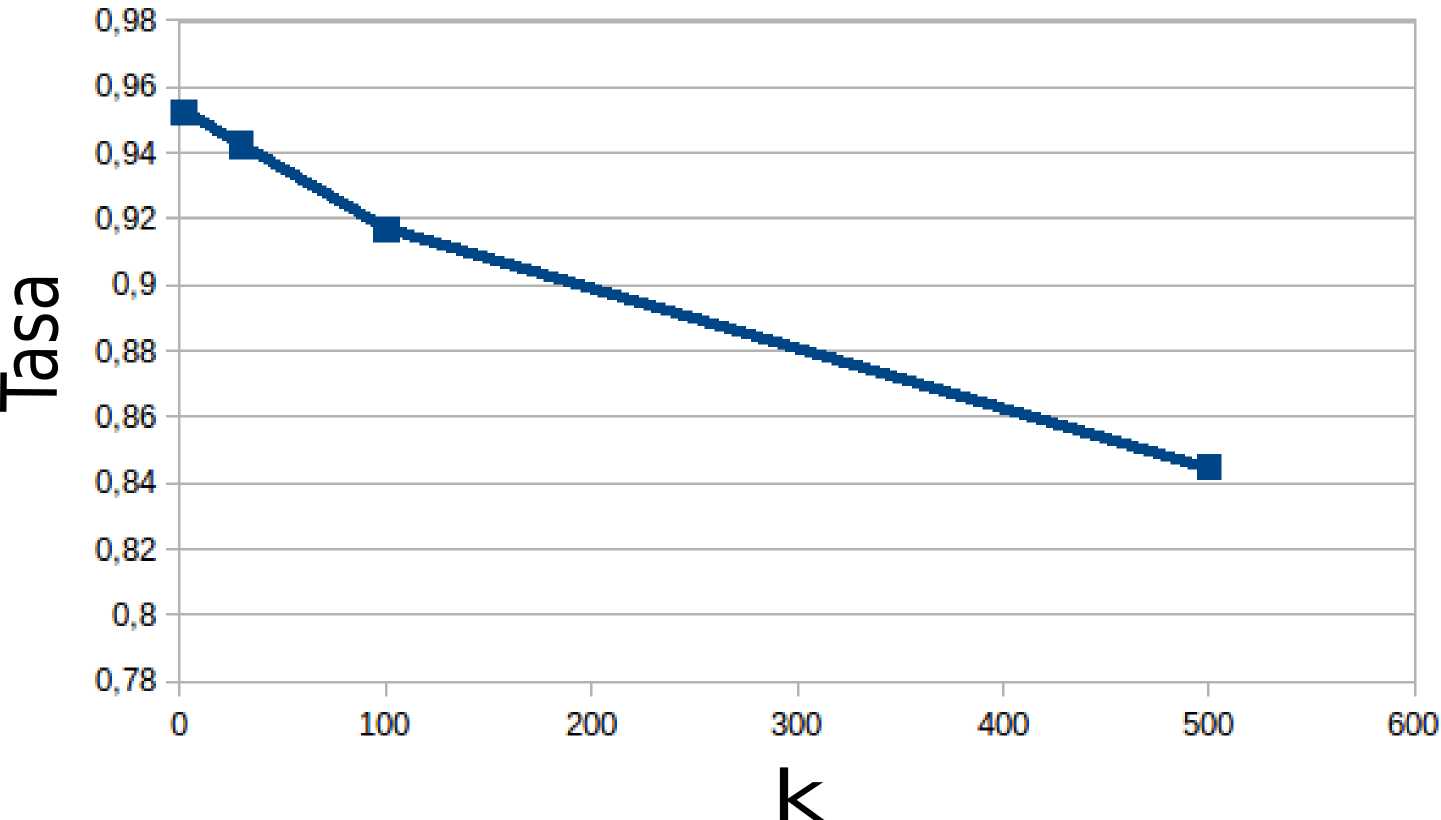
\includegraphics[scale=0.3]{Graficos/knnTasa2.png}
    \caption{Tasas para Knn variando k para dos particiones}
	\label{knnTasa2}
    \end{figure}
\bigskip
\bigskip
\bigskip






\begin{itemize}
\item Con K=10\\
\end{itemize}

\begin{center}

\begin{table}[H]
\centering
\begin{tabular}{|r|r|r|}
\hline
%\multicolumn{ 3}{|c|}{kNN variando k con K = 10} \\ \hline
\multicolumn{1}{|c|}{k} & \multicolumn{1}{c|}{Tiempo} & \multicolumn{1}{c|}{Tasa} \\ \hline
2 & 31056.21 & 0.96169 \\ \hline
30 & 34590.4  & 0.952262 \\ \hline
100 & 34449.695 & 0.93169 \\ \hline
500 & 37274.029 & 0.878833 \\ \hline
\end{tabular}
\caption{Resultados para Knn variando k para diez particiones}
\label{}
\end{table}
\end{center}

\bigskip
\bigskip
\bigskip

    \begin{figure}[H]
    \centering
    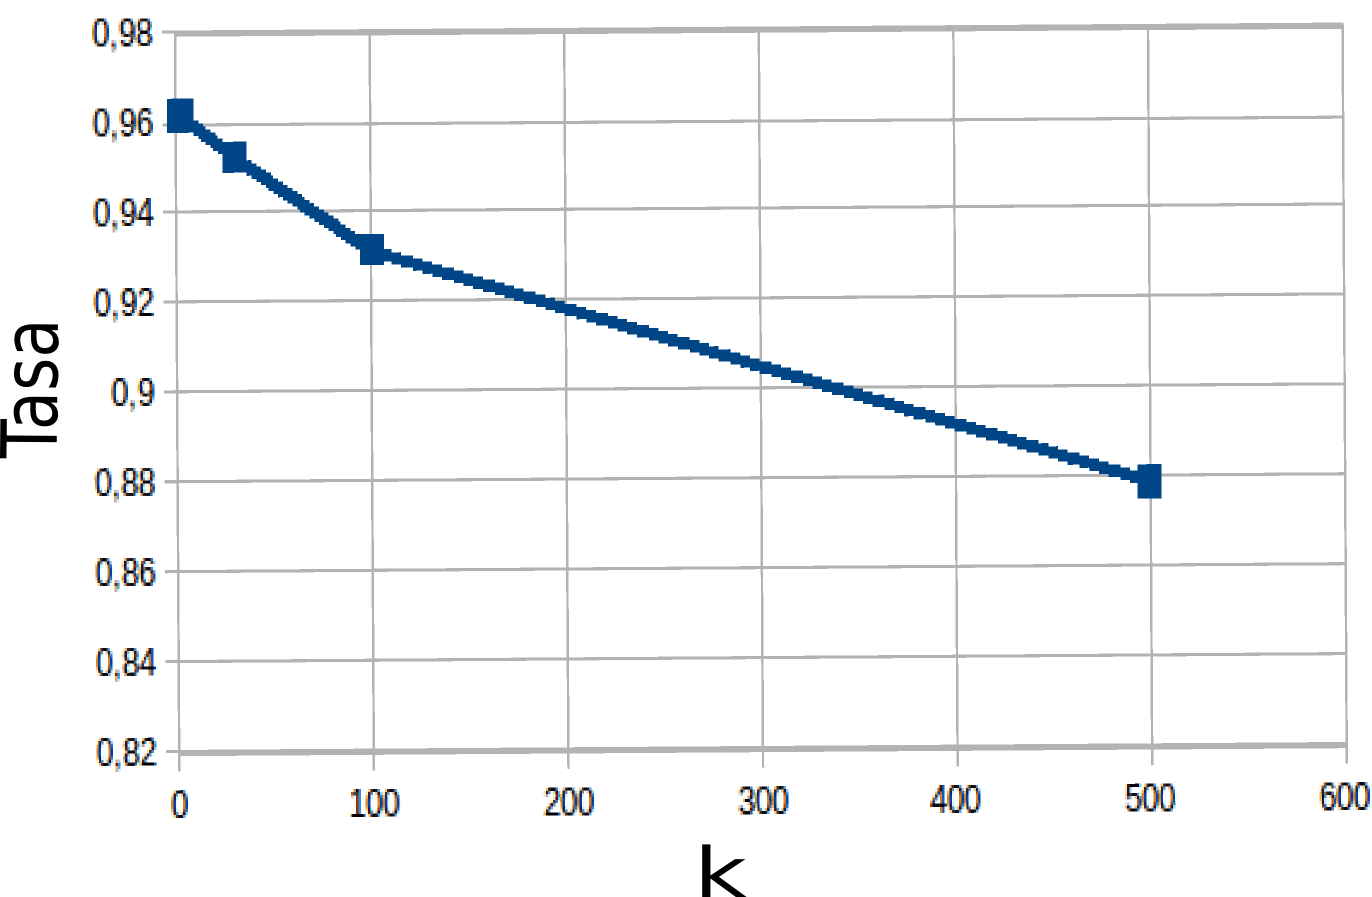
\includegraphics[scale=0.3]{Graficos/knnTasa10.png}
    \caption{Tasas para Knn variando k para diez particiones}
	\label{knnTasa10}
    \end{figure}
\bigskip
\bigskip
\bigskip




\begin{itemize}
\item Con K = 20\\
\end{itemize} 

\begin{table}[H]
\centering
\begin{tabular}{|r|r|r|}
\hline
\multicolumn{1}{|c|}{k} & \multicolumn{1}{c|}{Tiempo} & \multicolumn{1}{c|}{Tasa} \\ \hline
2 & 238893.923 & 0.962381 \\ \hline
30 & 263245.053 & 0.953167 \\ \hline
100 & 284027.496 & 0.933429 \\ \hline
500 & 313345.443 & 0.881381 \\ \hline
\end{tabular}
 \caption{Tasas para Knn variando k para veinte particiones}
\label{}
\end{table}
\bigskip
\bigskip
\bigskip

    \begin{figure}[H]
    \centering
    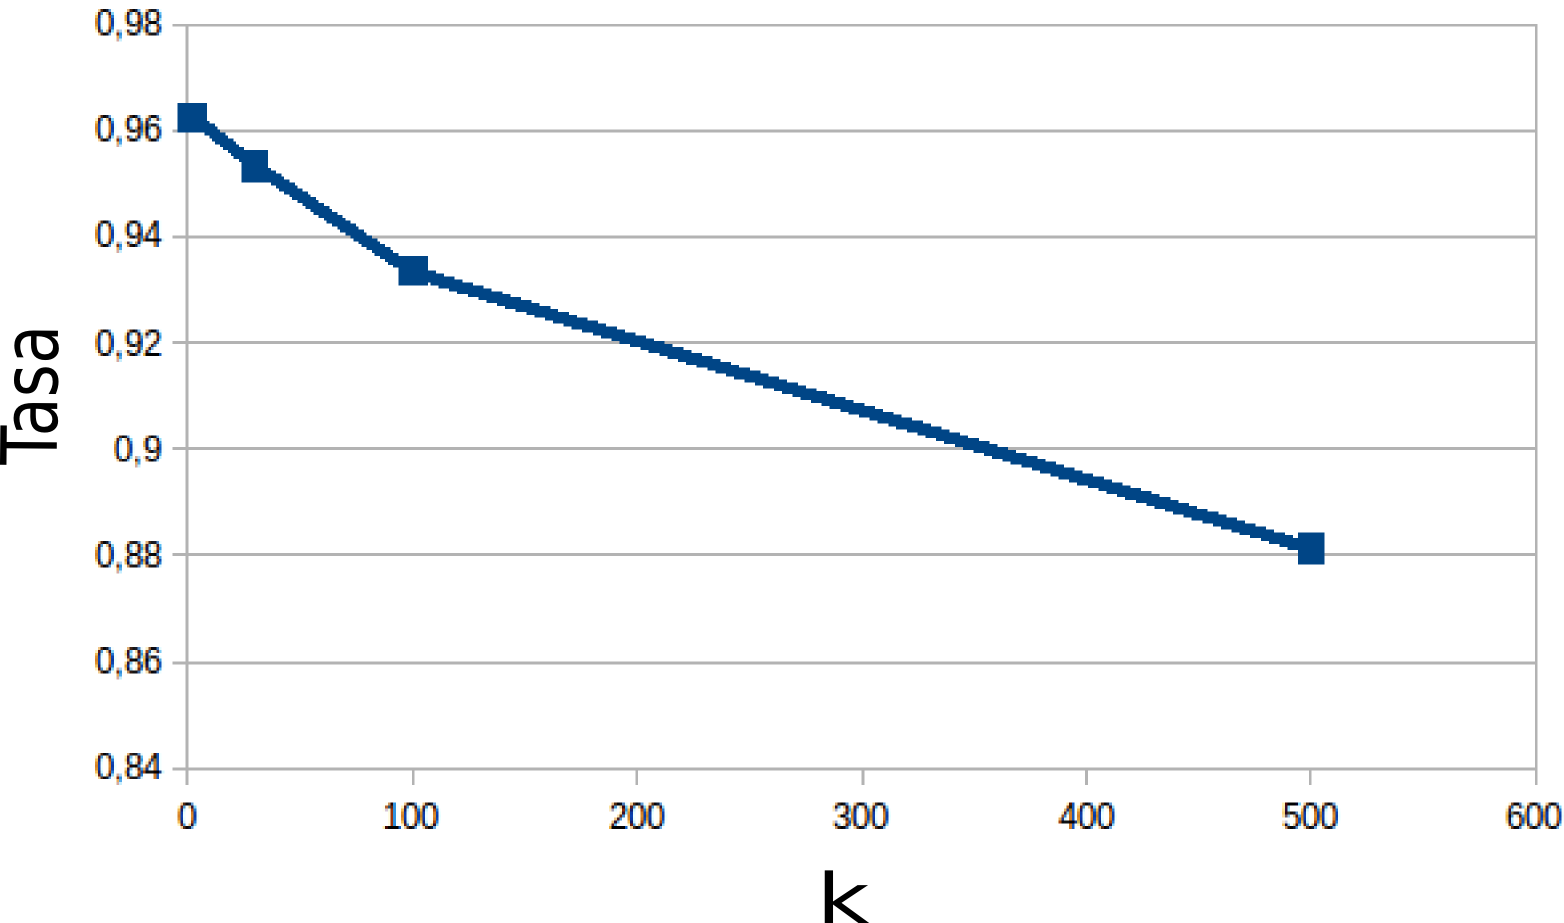
\includegraphics[scale=0.3]{Graficos/knnTasa20.png}
    \caption{Tasas para Knn variando k para veinte particiones}
	\label{knnTasa20}
    \end{figure}
\bigskip
\bigskip

En base a estos resultados se puede apreciar claramente la caída de la tasa en función de la cantidad de vecinos mas cercanos(k), y el aumento de tiempo de con el mismo.

\subsection{Experimento 2}
\subsubsection{Variando k}
A continuación, presentamos las tablas correspondientes a las tasas de reconocimiento y el tiempo de cómputo para los valores de $k$ elegidos en el desarrollo y para los distintos valores de $K$:
\newline
\newline
\centerline{Tasas:}
\newline
\centerline{
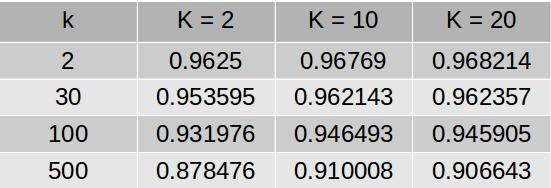
\includegraphics[scale=0.4]{Tablas/variandoktr.jpg}
}
\newline
\newline
\centerline{Tiempos:}
\newline
\centerline{
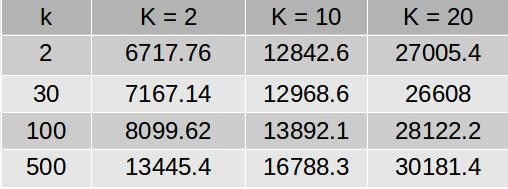
\includegraphics[scale=0.4]{Tablas/variandok.jpg}
}
\newline
\newline
Ahora vamos a comparar las tasas de PCA + KNN con las de KNN para los distintos $K$:
\newline
\newline
\centerline{
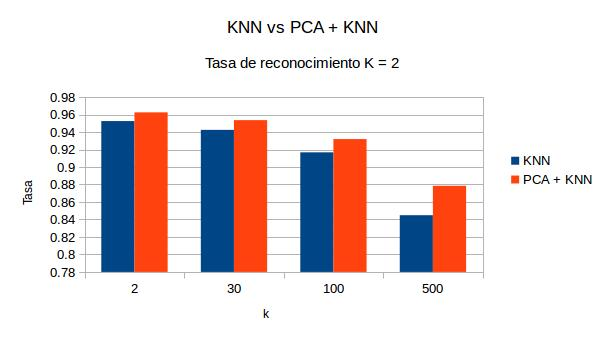
\includegraphics[scale=0.5]{Tablas/comtrK2.jpg}
}
\centerline{
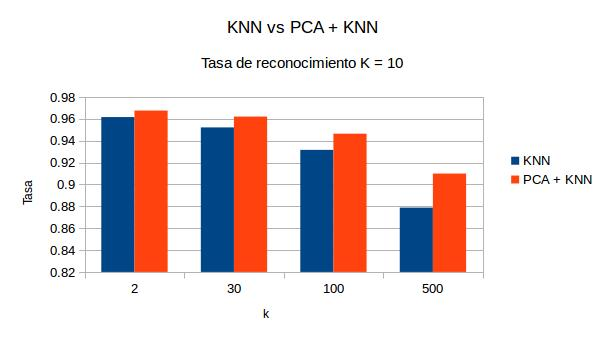
\includegraphics[scale=0.5]{Tablas/comtrK10.jpg}
}
\centerline{
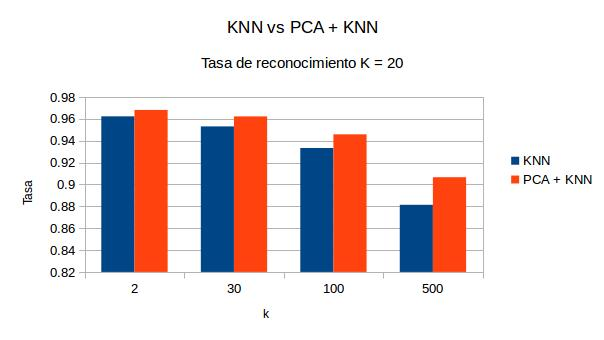
\includegraphics[scale=0.5]{Tablas/comtrK20.jpg}
}

Podemos observar como sorprendentemente PCA siempre supera a KNN, teóricamente esto no debería suceder.
\newline
\newline
A continuación presentamos un gráfico que compara los tiempos de KNN y PCA + KNN para $K = 2$ y $K = 10$, fijando $\alpha = 50$ en PCA y variando $k$:
\newline
\newline
\centerline{
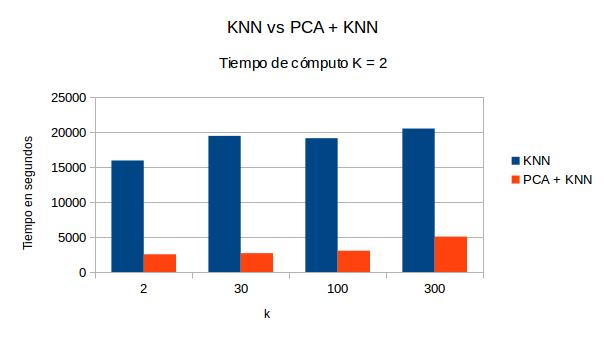
\includegraphics[scale=0.5]{Tablas/comtcK2.jpg}
}
\centerline{
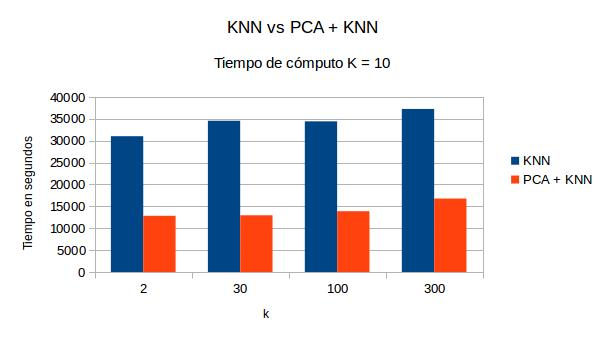
\includegraphics[scale=0.5]{Tablas/comtcK10.jpg}
}
\centerline{
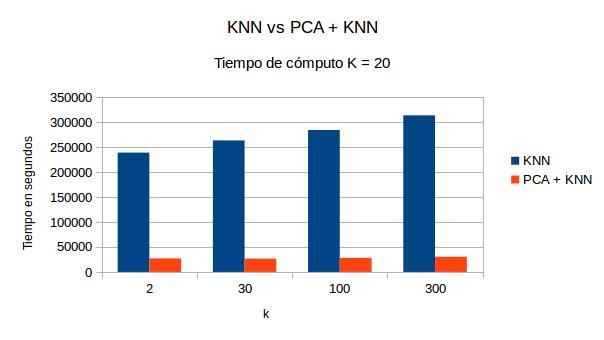
\includegraphics[scale=0.5]{Tablas/comtcK20.jpg}
}

En los gráficos muestran lo esperable que es que los tiempos de KNN son más grandes que los de PCA + KNN. Para los gráficos sobre $K = 20$, el tiempo de cómputo fue calculado de manera aproximada (multiplicando por 20 el tiempo que se tarda en procesar una partición de las 20) debido a que es demasiado grande. La tasa de reconocimiento en este caso tampoco es el promedio de las tasas porque no las tenemos, si no que es la tasa de reconocimiento de la partición particular que procesamos.

\subsubsection{Variando $\alpha$}
A continuación, presentaremos la tablas de los distintos K para los cuales corrimos PCA + KNN variando $\alpha$. En estos experimentos siempre vamos a estar utilizando el mismo valor de $k$ que va a ser 2 ya que fue elegido por ser el que maximiza la tasa de reconocimiento y minimiza el tiempo de cómputo.
\newline
\newline
\centerline{
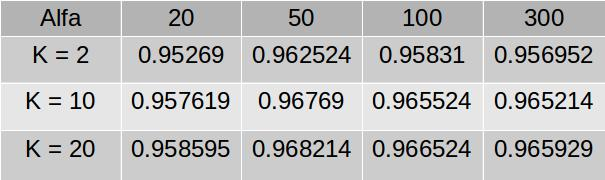
\includegraphics[scale=0.4]{Tablas/variandoAlfas.jpg}
}

Vemos como no se cumple la hipótesis que planteamos de que si aumentamos el valor de $\alpha$ entonces va a aumentar la tasa de reconocimiento ya que en los tres casos la tasa más alta está asociada a $\alpha = 50$ y es estrictamente mayor a las tasas con $\alpha = 100$ y $\alpha = 300$.
\newline Veamos los tiempos de cómputo asociados a estos valores de $\alpha$:
\newline
\newline
\centerline{
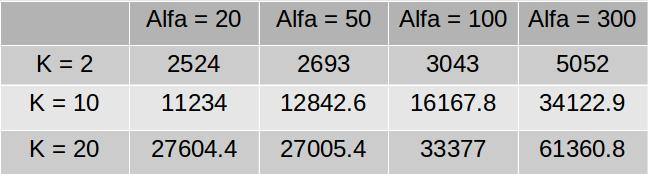
\includegraphics[scale=0.4]{Tablas/variandoalfatc.jpg}
}
\newline
\newline
Se puede ver en el gráfico como al hacer un aumento significativo en el $\alpha$ el tiempo de cómputo puede llegar a aumentar bastante. En los tres casos vemos que trabajar con $\alpha = 300$ requiere un tiempo de cómputo cercano al doble de lo que requiere con $\alpha = 20$. Esto significa que para valores cercanos de $\alpha$ el tiempo de cómputo no se va a ver afectado de manera significativa pero si realizamos aumentos grandes entonces es probable que el tiempo aumente de manera lineal.
\par Dado que nosotros queremos encontrar la mejor configuración tanto a nivel calidad de los resultados como tiempo de cómputo y vimos que las tasas variando $\alpha$ en 20, 50 100 y 300 son muy parecidas podríamos elegir $\alpha = 20$. De esta manera estaríamos minimizando el tiempo de cómputo y obteniendo una tasa de reconocimiento bastante alta. Sin embargo, en un contexto donde el tiempo de cómputo puede llegar a ser mucho más grande, por ejemplo porque estamos trabajando con un $K$ mucho mayor, porque contamos con bases de datos de mayor tamaño o por cualquier otro motivo, sería interesante poder reducir lo máximo que podamos al valor de $\alpha$. Es decir, nosotros sabemos que las tasas con $\alpha = 20, 50, 100$ y $300$ son muy similares, pero ¿cuanto más podemos disminuir $\alpha$ sin que la tasa de reconocimiento baje demasiado?. Para contestar esta pregunta decidimos disminuir el valor de $\alpha$ de una manera más drástica y ver que sucede. A continuación, se presentan las tasas de reconocimiento asociadas a los distintos $K$, para $\alpha = 5$:
\newline
\newline
\centerline{
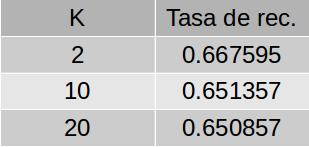
\includegraphics[scale=0.4]{Tablas/alfa5.jpg}
}
\newline
\newline
Los resultados demuestran que la diferencia de las tasas con respecto a los valores anteriores de $\alpha$ es claramente notable, lo que significa que deberíamos elegir un $\alpha$ entre 5 y 20. Es importante observar como al realizar una variación en el valor de $\alpha$, las tasas para los distintos valores de $K$ se mantienen muy parecidas. Esto significa que para reducir el tiempo de cómputo de la experimentación, podemos a tratar de encontrar este $\alpha$ utilizando $K = 2$ y lo que obtengamos también nos va a servir para $K = 10$ y $K = 20$. Probemos con $\alpha = $ 7, 13 y 16.
\newline
\newline
\centerline{
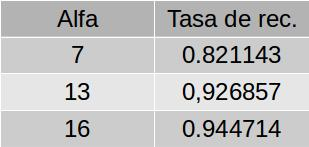
\includegraphics[scale=0.4]{Tablas/variandoalfaschicos.jpg}
}
\newline
\newline
Bien, la tabla muestra que para $\alpha = 13$ la tasa es $\approx 0.92$. Dado que con un valor de 7 estamos pasando el 0.8 y con 13 estamos pasando 0.92, tomando un valor de $\alpha = 10$ nuestra tasa va a ser $\approx 0.9$, lo cual es más que aceptable. Partimos de un valor de $\alpha = 50$ y experimentando, llegamos a que si bajamos ese valor a 10 entonces vamos a tener una tasa un poco peor pero igual muy buena y vamos a estar reduciendo mucho más la dimensión de nuestras muestras.


\newpage
\section{Discusión}
%Se incluirá aquí un análisis de los resultados obtenidos en la sección anterior (se analizará
%su validez, coherencia, etc.). Deben analizarse como míınimo los ítems pedidos en el
%enunciado. No es aceptable decir que “los resultados fueron los esperados”, sin hacer
%clara referencia a la teoría la cual se ajustan. Además, se deben mencionar los resul-
%tados interesantes y los casos “patológicos” encontrados.





\subsection{Hipótesis 1:}
Con respecto a la hipótesis 1, que establecía que corriendo cualquiera de los 2 métodos implementados(kNN y kNN+PCA) fijando k y $\alpha$, a mayor valor de K mayor porcentaje de tasas, procederemos primero a observar los resultados de kNN+PCA.\\ Comparando las tasas de efectivad resultantes de usar K=2 contra K=10 y K=20, se nota claramente que las de K=2 son menores que las de los otros dos valores de K. Esto es consecuencia principal del uso de la técnica de K-Fold Cross Validation, ya que con un valor K chico nuestra partición de la base de entrenamiento se divide en partes mas grandes, en consecuencia la longitud de la base de test tiende a ser igual a la base de entrenamiento. Dicho en otros términos, tenemos menos elementos en la base de entrenamiento para entrenar nuestro algoritmo y menos permutaciones sobre cuales elementos los consideramos parte del test. Esto es la principal causa de que con K=2 obtengamos los menores valores de la tasa de efectivida. Para que la tasa de efectividad tienda a 1, es necesario contar con una base lo más extensa posible. Y además al aumentar K, tenemos mas combinacion de particiones posibles y un entrenamiento más profundo. En este caso, la disminucion de la misma no se ve afectada por el valor que tome k y alpha. \\Hasta aqui la hipótesis se confirmaría, pero al analizar y comparar las tasas de K=10 contra K=20, observamos que aca si incide el valor que tome k. Para k con valores chicos, se ve una diferencia de la tasa cuando saltamos de K=10 a K=20, pero a medida que k aumenta, las tasas empiezan a comportarse de manera similar, teniendo vaivenes para algunos k, en el que la tasa de K=10 le gana a K=20 o viceversa. Ante esta situación, decidimos observar más detalladamente los datos de la experimentación y logramos ver que para k grandes y K=20, la muestra de las tasas de cada partición posee una mayor varianza, es decir que los valores tienen mayores fluctuaciones en comparación a la media de la muestra. Realizando un análisis más intensivo, deducimos que esto se debe a que a mayor valor de K, tengo mas elementos de entrenamiento, y a su vez a mayor valor de k, tengo más elemento que entrarán en la definición de vecinos más cercanos, pudiendo aqui encontrar elementos que no son del mismo label que el elemento en estudio y así alterar notablemente la tasa de efectividad en cada una de las particiones.\\
Como último dato, el valor de $\alpha$ no incide en las tasas de efectividad entre diferentes K, es decir, para un $\alpha$ fijo, a medida que se aumenta el valor de K, aumenta la tasa.\\
Con respecto al método de kNN, la elección de los K, se comporta de la misma manera y tiene las mismas consecuencias que en el método de kNN+PCA.
Finalmente se pordría concluir que la hipótesis queda parcialmente verificada, ya que la única parte que se refuto de la misma fue la parte de mantener k constante. Sobre esta particularidad de k, se continuará detallando en la discución del experimento 1.

\textbf{Análisis de tiempo de computo al variar K:}
 En el método de kNN+PCA, claramente se incrementa el tiempo de cómputo a medida que aumenta el valor de K, esto se debe a que el cálculo de la matriz de covarianza del entrenamiento domina gran parte del tiempo del metodo (sin contar la llamada a kNN). Dicha matriz se calcula de la siguiente forma: por ejemplo, si K=2, la matriz de entranamiento va a tener un tamaño de 21000x784, su transpuesta de 784x21000, entonces la matriz de covarianza se calcula multiplicando la transpuesta por la matriz de entrenamiento resultando siempre una matriz de 784x784. Para este caso de K, haremos 2 multiplicaciones de matrices de 784x21000 y 21000x784. Ahora bien, si suponemos que K=10, el procedimiento es el mismo, salvo que ahora, mi base de entrenamiento va a ser mas grande, por ende, su matriz también que en este caso va a tener tamaño de (42.000-42.000/10)x784 = 37800x784. Para este caso de K, haremos 10 multiplicaciones de matrices de 784x37.800 y 37.800x784. Al aumentar el valor de K, además de hacer más multiplicaciones por tener más particiones, las matrices aumentan de tamaño por lo explicado anteriormente. Para K=20 es el mismo procedimiento.\\
En el método de kNN, por ejemplo para K=2, voy a recorrer 2 veces la base de entrenamiento de 21000 dígitos para un base de test con la misma cantidad de dígitos. Para k=10, voy a recorrer 10 veces la base de train de 37.800 dígitos para una base de test de 4.200 digitos. Realizando un análisis más exhaustivo, para el primer caso de K=2, estariamos recorriendo 21.000 veces la base de 21.000 digitos, todo eso 2 veces lo que resultaria en 2*21.000*21.000 = 822.000.000 iteraciones. Para el caso de K=10, estariamos recorriendo 4200 veces la base de 37800 digitos, todo eso 10 veces lo que resultaria en 10*4.200*37.800 = 1.587.600.000 iteraciones, lo que implacarŕia un 93$\%$ más de iteraciones. Para K=20 pasa lo mismo.\\

 \subsection{Experimento 1:}

Podemos ver que en ningún caso se obtiene una tasa del 100$ \% $. Con un k chico se corre el riesgo de que los vecinos más cercanos no sean los correctos por una situación especial que pueda llegar a ocurrir, y entonces el dígito no sea reconocido, por ejemplo que justo el dígito en estudio este rodeado de k dígitos con otra caracterización. Se verifica empíricamente la hipótesis N$ ^{\circ} $ 2, con un k grande las tasas disminuyen apreciablemente. Esto se lo podemos atribuir a que hay una probabilidad no despreciable de que un dígito a reconocer este mas cercano a un dígito con distinta caracterizacón que a uno con igual. No es una cuestión de falta de dígitos iguales al que se esta reconociendo. Por ejemplo al tomar 500 vecinos mśs cercanos, no es que no halla sido posible tomar a estos 500 como el dígito a reconocer por falta de este ultimo en la matriz de train, sino que en lugar de tomarse un dígito con igual caracterización, se toma uno con distinta, pero más cercano.

También podemos ver que al incrementar k se obtiene un tiempo mayor. Esto se debe a que el algoritmo de knn en cada paso, recorre un vector de tamaño k donde se encuentran los mas cercanos, y lo va ir actualizando. 



 \subsection{Experimento 2:}
\subsubsection{Variando k}
Al realizar las variaciones de $k$ propuestas en el desarrollo obtuvimos distintas tasas de reconocimiento que, como podemos observar en la primera tabla, van empeorando a medida que aumenta el $k$. Esto pasa porque, aunque estemos haciendo PCA primero, luego vamos a estar aplicando KNN y ya vimos que cuando aplicamos KNN y aumentamos el valor de $K$, las tasas empeoran, independientemente del preprocesamiento de los datos.
\subsubsection{Variando $\alpha$}
En los experimentos vimos que nuestra hipótesis de que al aumentar el valor de $\alpha$ ibamos a estar aumentando la tasa de reconocimiento es falsa. Sin embargo, cuando bajamos de $\alpha = 50$ a $\alpha = 5$ pudimos notar una diferencia importante en la tasa de reconocimiento. Una posible explicación a lo que está sucediendo es que, si bien matemáticamente tiene sentido pensar que deberíamos tener tasas de reconocimiento más altas al aumentar $\alpha$ (porque agrandamos nuestra base en la cual expresamos nuestros datos), nosotros estamos implementando todo esto en una computadora. Esto significa que todo lo que hacemos tiene cierto error y que ese error puede ir incrementandose. 
\par Los autovectores por ejemplo, los calculamos mediante el método de la potencia, pero no debemos olvidarnos que el método de la potencia se basa en aproximar un límite. Esto quiere decir que los autovalores y autovectores que estamos calculando, en realidad no van a ser exactamente los que queremos obtener. En la experimentación vimos que a partir de un cierto valor, ya no tiene sentido seguir aumentando $\alpha$ porque las tasas dan muy similares (incluso peores) y el tiempo de cómputo aumenta. Tranquilamente lo que podría estar pasando es que, los primeros autovectores que estemos calculando tengan menos error (porque el método de la potencia para ellos converge más rapidamente) y a medida que se va aumentando la cantidad de autovectores, el error que se produce al calcular cada uno de ellos es cada vez más grande. Esto explicaría lo que pasa en nuestros resultados porque los primeros autovectores de la base son los que estarían aportando más información (porque son los que menos error tendrían) y a partir de un punto, el error es tan grande que ya no aporta información confiable y puede ocurrir entonces que la tasa de reconocimiento empeore.



\subsection{Competencia Kaggle}
Para realizar nuestro submission en la página de Kaggle, a la competencia de Digit Recognizer, modificamos levemente el codigo de nuestro programa. El mismo se encuentra en la carpeta Kaggle. Las modificaciones se deben a que en este caso, la base de test proporcionada por la página no tiene labels, no utilizamos el método de K-Fold Cross Validation, la funcion kNN ahora tiene que devolver las predicciones de los dígitos, entre otras cosas.\\
Luego de toda la experimentación concluímos que los mejores parámetros, en cuanto tiempo y eficacia, para correr el programa son algún k y $\alpha$ cercanos a:
\begin{itemize}
\item $\alpha$ = 50
\item $k$ = 2
\end{itemize}

A continuación probaremos con valores cercanos a estos parámetros para estudiar la efectividad que nos proporciona el sistema de Kaggle.
\begin{itemize}
	\item Con k=2 y $\alpha$=50, tuvimos una efectividad de 0.96686 con un tiempo de computo de 1338.35 
	\item Con k=3 y $\alpha$=50, tuvimos una efectividad de 0.96857 con un tiempo de computo de 1454.45.
	\item Con k=3 usando solo kNN, tuvimos una efectividad de 0.97200 con un tiempo de computo de 12691.6.
	\item Con k=4 y $\alpha$=50, tuvimos una efectividad de 0.97286 con un tiempo de computo de 1654.71.
\end{itemize}
\newpage
\section{Conclusiones}
%Esta sección debe contener las conclusiones generales del trabajo. Se deben mencionar
%las relaciones de la discusión sobre las que se tiene certeza, junto con comentarios
%y observaciones generales aplicables a todo el proceso. Mencionar también posibles
%extensiones a los métodos, experimentos que hayan quedado pendientes, etc.

Podemos concluir que el método de knn utilizando la norma dos como distancia entre dígitos tiene un margen de error para reconocer a los mismos, lo cual hace que en algunas situaciones no se pueda utilizar, ya que no es aceptable una equivocación. El error de este ultimo método se debe en parte a la cercanía en norma dos de dígitos distintos, pero también en parte a los errores numéricos que se propagan al hacer operaciones aritméticas en la computadora. Este hecho se pone en evidencia al obtener que con el método de pca se obtienen tasas de reconocimiento mas altas. 

Este ultimo método resulta muy efectivo para el reconocimiento de dígitos. En teoría de ya que toma un tiempo considerablemente menor, y 

\newpage
\section{Apéndices}

%\usepackage[ruled,vlined]{algorithm2e}

\parindent = 0 pt
\parskip = 5 pt

\addtolength{\topmargin}{-1cm}
\addtolength{\textheight}{1cm}

\newcommand{\real}{\mathbb{R}}
\newcommand{\kknn}{k}
\newcommand{\kpca}{\alpha}
\newcommand{\kkfold}{K}

%En el apéndice A se incluirá el enunciado del TP. En el apéndice B se incluirán los
%códigos fuente de las funciones relevantes desde el punto de vista numérico. Resultados
%que valga la pena mencionar en el trabajo pero que sean demasiado específicos para
%aparecer en el cuerpo principal del trabajo podrán mencionarse en sucesivos apéndices
%rotulados con las letras mayusculas del alfabeto romano. Por ejemplo: la demostración
%de una propiedad que aplican para optimizar el algoritmo que programaron para resolver
%un problema.

\subsection*{Apéndice A:}

\begin{center}
\begin{tabular}{r|cr}
 \begin{tabular}{c}
{\large\bf\textsf{\ M\'etodos Num\'ericos\ }}\\ 
Primer Cuatrimestre 2015\\
{\bf Trabajo Pr\'actico 2}\\
\end{tabular} &
\begin{tabular}{@{} p{1.6cm} @{}}

\includegraphics[width=1.6cm]{logodpt.jpg}
\end{tabular} &
\begin{tabular}{l @{}}
 \emph{Departamento de Computaci\'on} \\
 \emph{Facultad de Ciencias Exactas y Naturales} \\
 \emph{Universidad de Buenos Aires} \\
\end{tabular} 
\end{tabular}
\vskip 10pt
\textbf{\Large }
\end{center}

\vskip 10pt
\hrule
\vskip 5pt

{\bf\noindent Introducci\'on}

Uno de los momentos de mayor tensi\'on durante un cuatrimestre se genera en \'epocas de parciales. El d\'ia del examen, luego de entregar la resoluci\'on del mismo, suele aparecer esa inmanejable incertidumbre en los alumnos: \emph{?`entregu\'e todas las hojas?}, \emph{?`consider\'e el caso particular de $\beta = 0$?}, \emph{?`por qu\'e mi compa\~nero puso verdadero, si yo encontr\'e un contraejemplo?} Desde el lado del docente, la dificultad radica en corregir un gran volumen de ejercicios t\'ecnicamente complejos en un tiempo acotado, buscando deducir en base a informaci\'on limitada si el alumno comprendi\'o o no el tema. 

Estos dos factores llevaron a la conformaci\'on de una comisi\'on interclaustro de docentes y alumnos, para quienes resguardamos su identidad, a proponer como soluci\'on el desarrollo de una herramienta autom\'atica de correcci\'on de ex\'amenes, con el fin de reducir los tiempos en la devoluci\'on de los mismos. Para evitar suspicacias respecto de las correcciones, se propuso dividir el problema en varias etapas y que el sistema sea desarrollado por alumnos, contando desde ya con la validaci\'on de los docentes. La primera etapa del proyecto consiste en desarrollar una herramienta que permita autom\'aticamente identificar d\'igitos manuscritos, a ser aplicada a una digitalizaci\'on de cada examen, y cuyo post-procesamiento involucrar\'a darle sem\'antica y reglas a la informaci\'on obtenida.

Como es de esperar, el \'exito de la herramienta depende inevitablemente de disponer de un buen reconocedor de d\'igitos manuscritos. Para semejante responsabilidad, dado el gran nivel mostrado durante el comienzo del cuatrimestre, la comisi\'on asesora ha decidido elegir a los alumnos de M\'etodos Num\'ericos para llevar adelante el desarrollo.

{\bf\noindent Objetivos y Metodolog\'ia}

Como instancias de entrenamiento, se tiene una base de datos de $n$ im\'agenes de $M \times M$ p\'ixeles, las cuales se encuentran etiquetadas con el d\'igito, 0-9, al que corresponden. Definimos como $m = M \times M$ al n\'umero total de p\'ixeles de una imagen. Asumiremos tambi\'en que las im\'agenes se encuentran en escala de grises (cada pixel corresponde a un valor entre 0 y 255, indicando la intensidad del mismo) y que el etiquetado no contiene errores. El objetivo del trabajo consiste en utilizar la informaci\'on de la base de datos para, dada una nueva imagen de un d\'igito sin etiquetar, determinar a cu\'al corresponde teniendo en cuenta factores de calidad y tiempo de ejecuci\'on requeridos.

Una primera aproximaci\'on es utilizar el conocido algoritmo de \emph{$\kknn$ Vecinos m\'as Cercanos} ($kNN$, por su nombre en ingl\'es). En su versi\'on m\'as simple, este algoritmo considera a cada objeto de la base de entrenamiento como un punto en el espacio, para el cual se conoce a qu\'e clase corresponde (en nuestro caso, qu\'e d\'igito es). Luego, al obtener un nuevo objeto que se busca clasificar simplemente se buscan los $\kknn$ vecinos m\'as cercanos y se le asigna la clase que posea el mayor n\'umero de repeticiones dentro de ese subconjunto, es decir, la moda. Con este objetivo, podemos representar a cada imagen de nuestra base de datos como un vector $x_i \in \real^{m}$, con $i = 1,\dots,n$, y de forma an\'aloga interpretar las im\'agenes a clasificar mediante el algoritmo $kNN$.

Sin embargo, el algoritmo del vecino m\'as cercano es sensible a la dimensi\'on de los objetos a considerar y, a\'un aplicando t\'ecnicas de preprocesamiento, puede resultar muy costoso de computar. Teniendo en cuenta esto, una alternativa interesante de preprocesamiento que busca reducir el tama\~no de los elementos a considerar es el m\'etodo de \emph{An\'alisis de Componentes Principales} (PCA, por su sigla en ingl\'es), que consiste en lo siguiente. Para $i = 1,\ldots, n$, recordar que $x_i \in \real^{m}$ la $i$-\'esima imagen de nuestra base de datos almacenada por filas en un vector, y sea $\mu = (x_1 + \ldots + x_n)/n$ el promedio de las im\'agenes. Definimos $X\in\real^{n\times m}$ como la matriz que contiene en la $i$-\'esima fila al vector $(x_i - \mu)^{t}/\sqrt{n-1}$, y $$A=U \Sigma V^t$$ a su descomposici\'on en valores singulares, con $U\in\real^{n\times n}$ y $V\in\real^{m\times m}$ matrices ortogonales, y $\Sigma\in\real^{n\times m}$ la matriz diagonal conteniendo en la posici\'on $(i,i)$ al $i$-\'esimo valor singular $\sigma_i$. Siendo $v_i$ la columna $i$ de $V$, definimos para $i = 1,\ldots,n$ la \textsl{transformaci\'on caracter\'istica} del d\'igito $x_{i}$ como el vector $\mathbf{tc}(x_i) = (v_1^t\, x_i, v_2^t\, x_i,\ldots,v_{\kpca}^t\, x_i) \in\real^{\kpca}$, donde $\kpca \in\{1,\ldots,m\}$ es un par\'ametro de la implementaci\'on. Este proceso corresponde a extraer las $\kpca$ primeras \textit{componentes principales} de cada imagen. La intenci\'on es que $\mathbf{tc}(x_i)$ resuma la informaci\'on m\'as relevante de la imagen, descartando los detalles o las zonas que no aportan rasgos distintivos. Dada una nueva imagen $x$ de un d\'igito, se calcula $\mathbf{tc}(x)$ y se compara con $\mathbf{tc}(x_i)$, para $i = 1,\ldots, n$, utilizando alg\'un criterio de clasificaci\'on adecuado, como por ejemplo $kNN$.

Finalmente, nos concentramos en la evaluaci\'on de los m\'etodos. Dado que necesitamos conocer a qu\'e d\'igito corresponde una imagen para poder verificar la correctitud de la clasificaci\'on, una alternativa es particionar la base de entrenamiento en dos, utilizando una parte de ella en forma completa para el entrenamiento y la restante como test, pudiendo as\'i corroborar la predicci\'on realizada. Sin embargo, realizar toda la experimentaci\'on sobre una \'unica partici\'on de la base podr\'ia resultar en una incorrecta estimaci\'on de par\'ametros, como por ejemplo el conocido \emph{overfitting}. Luego, se considera la t\'ecnica de \emph{cross validation}, en particular el \emph{$\kkfold$-fold cross validation}, para realizar una estimaci\'on de los par\'ametros del modelo que resulte estad\'isticamente m\'as robusta.\\ 

{\bf\noindent Enunciado}

Se pide implementar un programa en \verb+C+ o \verb-C++- que lea desde archivos las im\'agenes de entrenamiento correspondientes a distintos d\'igitos y que, utilizando los m\'etodos descriptos en la secci\'on anterior, dada una nueva imagen de un d\'igito determine a qu\'e n\'umero pertenece. Para ello, el programa deber\'a implementar el algoritmo de $kNN$ as\'i como tambi\'en la reducci\'on de dimensi\'on previa utilizando PCA.  

Con el objetivo de obtener la descomposici\'on en valores singulares, se deber\'a implementar el m\'etodo de la potencia con deflaci\'on para la estimaci\'on de autovalores/autovectores de la matriz de covarianza. En este contexto, la factibilidad de aplicar este m\'etodo es particularmente sensible al tama\~no de las im\'agenes de la base de datos. Por ejemplo, considerar im\'agenes en escala de grises de $100 \times 100$ p\'ixeles implicar\'ia trabajar con matrices de tama\~no $10000 \times 10000$. Se pide tener en cuenta este factor durante el desarrollo y analizar c\'omo afecta (si es que lo hace) en el desarrollo del trabajo. 

Consideramos la base de datos MNIST, en la versi\'on disponible en \emph{Kaggle}. Esta base contiene un conjunto de datos de entrenamiento de 42.000 d\'igitos manuscritos en escala de grises y con $M = 28$. A su vez, provee un conjunto de datos de test de 28.000 d\'igitos, de similares caracter\'isticas, pero sin el correspondiente etiquetado. En base a estos datos, se pide separar el procedimiento en dos etapas. 

La primera de ellas consiste en realizar un estudio experimental con los m\'etodos propuestos sobre la base de entrenamiento y utilizando la t\'ecnica de \emph{$\kkfold$-fold cross validation} mencionada anteriormente. Para esta \'ultima tarea en particular, se recomienda leer y utilizar la rutina \verb+cvpartition+ provista por MATLAB. Llamamos $\kknn$ a la cantidad de vecinos a considerar en el algoritmo $kNN$, $\kpca$ a la cantidad de componentes principales a tomar y $\kkfold$ a la cantidad de particiones consideradas para el cross-validation. La calidad de los resultados obtenidos ser\'an analizados considerando la tasa de efectivdad lograda, es decir, la cantidad d\'igitos correctamente clasificados respecto a la cantidad total de casos analizados. En funci\'on de la experimentaci\'on se piden como m\'inimo los siguientes experimentos:
\begin{itemize}
\item Analizar el comportamiento y la factibilidad de aplicar el algoritmo $kNN$ para un rango razonable de valores distintos de $\kknn$, analizando el compromiso entre el tiempo de ejecuci\'on y la calidad de los resultados obtenidos. Es posible, como experimento opcional, considerar alguna t\'ecnica alternativa de preprocesamiento de la informaci\'on en caso de ser necesario (y, desde ya, que no sea PCA). 
\item Analizar la calidad de los resultados obtenidos al combinar PCA con $kNN$, para un rango amplio de combinaciones de valores de $\kknn$ y $\kpca$. Considerar en el an\'alisis tambi\'en el tiempo de ejecuci\'on.
\item Realizar los experimentos de los items anteriores para al menos dos valores distintos de $\kkfold$. Justificar el por qu\'e de la elecci\'on de los mismos.
\item En base a los resultados obtenidos para ambos m\'etodos, seleccionar aquella combinaci\'on de par\'ametros que se considere la mejor alternativa, con su correspondiente justificaci\'on, y compararlas entre s\'i y sugerir un m\'etodo para su utilizaci\'on en la pr\'actica.
\end{itemize}

Finalmente, y con los par\'ametros seleccionados en la fase experimental, ejecutar el m\'etodo seleccionado sobre el conjunto de datos de test, utilizando como entrenamiento los 42.000 d\'igitos comprendidos en el conjunto de entrenamiento. Analizar el tiempo de c\'omputo requerido. Dado que la c\'atedra no posee la informaci\'on sobre a qu\'e d\'igito corresponde cada imagen (y la idea no es graficar uno por uno y obtenerlo a mano), se sugiere a cada grupo participar en la competencia \emph{Digit Recognizer} actualmente activa en \emph{Kaggle} realizando el/los env\'ios que consideren apropiados y reportar en el informe los resultados obtenidos.\\

Puntos opcionales (no obligatorios)

\begin{itemize}
\item Mostrar que si tenemos la descomposici\'on $A = U\Sigma V^t$, $V$ es la misma matriz que obtenemos al diagonlizar la matriz de covarianzas.
\item Realizar experimentos utilizando d\'igitos manuscritos creados por el grupo, manteniendo el formato propuesto.\footnote{Notar que en la base original las figuras est\'an rotadas y es blanco sobre negro, y no al rev\'es.} Reportar resultados y dificultades encontradas.
\item Implmenentar alguna mejora al algoritmo de $kNN$.
\end{itemize}

{\bf\noindent Programa y formato de archivos}

Se deber\'an entregar los archivos fuentes que contengan la resoluci\'on del trabajo pr\'actico. El ejecutable tomar\'a tres par\'ametros por l\'inea de comando, que ser\'an el nombre del archivo de entrada, el nombre del archivo de salida, y el m\'etodo a ejectutar (0: $kNN$, 1: PCA + $kNN$).
	

Asumimos que la base de datos de im\'agenes de entrenamiento se llama \verb+train.csv+ y que la base de test \verb+test.csv+, y que ambas siguen el formato establecido por la competencia. Para facilitar la experimentaci\'on, el archivo de entrada con la descripci\'on del experimento tendr\'a la siguiente estructura: 

\begin{itemize}
\item La primera l\'inea contendr\'a el path a la(s) base(s) de datos, $\kknn$, $\kpca$ y $\kkfold$.
\item Luego, habra $\kkfold$ l\'ineas de 42.000 valores, uno por cada muestra de la base de entrenamiento, donde un 1 indicar\'a que esa muestra se considera parte del entrenamiento, y un 0 que se considera parte del test. Luego, de esta forma se pueden codificar las particiones realizadas por el \emph{$\kkfold$-fold cross validation}.
\end{itemize}

El archivo de salida obligatorio tendr\'a para cada partici\'on que figure en el archivo de entrada el vector soluci\'on con los $\kpca$ valores singulares de mayor magnitud, con una componente del mismo por l\'inea. Adem\'as, el programa deber\'a generar un archivo, cuyo formato queda a criterio del grupo, indicando la tasa de reconocimiento obtenida para cada partici\'on. Adicionalmente, se generar\'a un archivo que concatene la extension \verb+.csv+ al segundo valor recibido como par\'ametro del programa, que escribir\'a la predicci\'on realizada sobre la base de test en el formato requerido por la competencia siguiendo el formato establecido por las reglas de la competencia.

Junto con el presente enunciado, se adjunta una serie de scripts hechos en \verb+python+ y un conjunto instancias de test que deber\'an ser utilizados para la compilaci\'on y un testeo b\'asico de la implementaci\'on. Se recomienda leer el archivo \verb+README.txt+ con el detalle sobre su utilizaci\'on.

\vskip 0.5 cm
\hrule
\vskip 0.1 cm

{\bf Sobre la entrega}
\begin{itemize}
\item \textsc{Formato electr\'onico:} Jueves 14 de Mayo de 2015, \underline{hasta las 23:59 hs.}, enviando el trabajo
(\texttt{informe} + \texttt{c\'odigo}) a \texttt{metnum.lab@gmail.com}. El \texttt{asunto} del email debe comenzar con el texto \verb|[TP2]| seguido
de la lista de apellidos de los integrantes del grupo. Ejemplo: \texttt{[TP2] Acevedo, Miranda, Montero}
\item \textsc{Formato f\'isico:} Viernes 15 de Mayo de 2015, de 17:30 a 18:00 hs.
\end{itemize}

\newpage

\subsection{Apéndice B:}

\begin{verbatim}

double ObtenerAutovalorMayor(Matriz<double> &A, Matriz<double>& v0){

    double lambda= normaInf(v0);
    double normalizar= norma2(v0);

    for(int i = 0; i < v0.filas(); i++){ v0[i][0] = v0[i][0]/normalizar;}

    Matriz<double> v1(v0.filas(),1);
    int i = 0;
    for(;i<3000 ;i++)
    {

        v1= A* v0;

        lambda= normaInf(v1)/normaInf(v0);

        normalizar = norma2(v1);

        for(int j = 0; j < v1.filas(); j++){ v1[j][0] = v1[j][0]/normalizar; }
        if(haypocadif(v0, v1)){break;}
        v0=v1;
    }

    return lambda;
}

vector<double> metodoPotencias(Matriz<double>& A, unsigned int alpha, Matriz<double>& P, 
Matriz<double>& v){

    vector<double> autovalores;

    for(int i=0;i<alpha;i++)
    {
        double autovalori= ObtenerAutovalorMayor(A,v);

        autovalores.push_back(autovalori);

        for(int j=0;j<A.columnas();j++){ P[j][i]=v[j][0]; }

        Matriz<double> vt(1, v.filas());

        vt= v.traspuesta();

        Matriz<double> prod(v.filas(),v.filas());
        prod= v*vt*autovalori;

        A =A - prod;
    }

    return autovalores;
}





\end{verbatim}
\newpage
%\section{Referencias}
%Es importante incluir referencias a libros, artículos y páginas de Internet consultados
%durante el desarrollo del trabajo, haciendo referencia a estos materiales a lo largo del
%informe. Se deben citar también las comunicaciones personales con otros grupos.


\begin{thebibliography}{1}
\bibitem{Sistema Bandas} Faires, J. D. and Burden, R. L. Numerical methods, 3rd ed. Publisher: Brooks Cole, p. 331, 2002.
\bibitem{Eliminación Gaussiana}Faires, J. D. and Burden, R. L. Análisis Numérico, 7rd ed. p. 345, 2011.
	\bibitem{Factorización LU} Fires, J. D. and Burden, R. L. Numerical methods, 3rd ed. Publisher: Brooks Cole, p. 271, 2002.
	\bibitem{ShermanMorrison} Golub, G. H. and Van Loan, C. F. Matrix Computations, 3rd ed. Baltimore, MD: Johns Hopkins, p. 51, 1996.
\end{thebibliography}


\newpage
\bibliographystyle{plain}

\end{document}
